\chapter{The Origin of the Name}
\label{ch:appendix-name}
When one builds a time machine and travels back in time he or she can change the course of history.
Even a small change in the historic events that lead to todays reality can have a big impact on the progression of time and can lead to a completely different reality from the one we know.
This is due to a phenomenon called \textit{the butterfly effect}.

This phenomenon plays a large role in the plot of the 1989 movie \textit{Back to the Future Part II}.
In that movie Marty McFly, the protagonist, travels forward in time with his friend Doc Brown where they discover a very different reality from the one they are used to.
This can be attributed to their actions in the previous film where they travelled \textit{back} in time.
Their previous time travel caused reality to diverge from the path it originally followed and sends it instead down an alternative timeline.

\begin{figure}[h!]
  \centering
    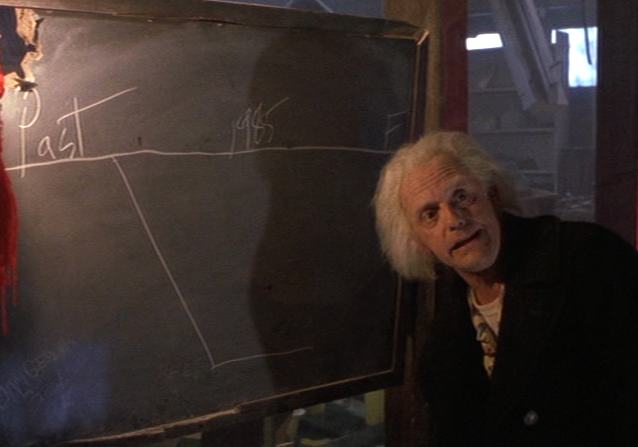
\includegraphics[width=0.6\textwidth]{doc-brown}
  \caption{Doc Brown explains alternative timelines for Marty}
  \label{fig:history-data-table}
\end{figure}

This is similar to what happens when a user creates a clone database.
The clone diverges from the original master database as the user executes different queries than are executed on the master.
The similarities between this behaviour and the plot in \textit{Back to the Future Part II} was the inspiration for the name \textit{Marty}, which is the same as the name of the protagonist in the film.